\documentclass[a4paper, 12pt]{article}

\usepackage[left=25mm, top=20mm, right=10mm, bottom=25mm, nohead, nofoot]{geometry}

\usepackage{cmap}
\usepackage[T2A]{fontenc}
\usepackage[utf8]{inputenc}
\usepackage[english, russian]{babel}

%Графика
\usepackage{graphicx}
\usepackage{float}%"Плавающие" картинки
\usepackage{wrapfig}%Обтекание фигур (таблиц, картинок и прочего)
\graphicspath{{./images/}}

% Математика
\usepackage{amsmath,amsfonts,amssymb,amsthm,mathtools} 

%Title Page
\title{ЛАБОРАТОРНАЯ РАБОТА № 1 \\
Моделирование механических систем
}
\author{Вариант 11 \\ Машуров Владимир БПМ-19-3}

\setcounter{page}{0}

\begin{document}
\maketitle
\thispagestyle{empty}
\newpage
\tableofcontents

\section{Моделирование механической системы масса-пружина}

Дана система: $M\dot{x} + B\dot{x} + kx = f(t)$ 

\textbf{Задание 1.1 } \\
Применив преобразование Лапласа (с нулевыми начальными условиями) найдите передаточную функцию модели: $ G(s) = \frac{X(s)}{F(s)} $

Найдём соотношение из которого получим G(t):


$$M\dot{x}(t) + B\dot{x}(t) + kx(t) = f(t) \; \; \; \frac{d}{dt} = \lambda $$

$$ M\lambda^2x(t) + B\lambda x(t) + kx(t) = f(t) $$

$$ (M\lambda^2 + B\lambda + k)x(t) = f(t) $$

$$ \frac{x(t)}{f(t)} = \frac{1}{M\lambda^2 + B\lambda + k} $$

Отсюда

$$ G(s) = \frac{X(s)}{F(s)} = \mathcal{L} \bigg( \frac{x(t)}{f(t)} \bigg) = \frac{\mathcal{L}(\tilde{x}(t))}{\mathcal{L}(\tilde{f}(t))} = $$
$$ = \frac{\mathcal{L}(1)}{\mathcal{L}(M\lambda^2 + B\lambda + k)} =  \frac{1}{s} \cdot \frac{s}{M\lambda^2 + B\lambda + k} = \frac{1}{M\lambda^2 + B\lambda + k} $$

\textbf{Задание 1.2 } \\
Перепишите уравнение (1) в форму вход-состояние-выход.

$$M\dot{x}(t) + B\dot{x}(t) + kx(t) = f(t) \; \; \; \frac{d}{dt} = \lambda $$

$$ \begin{cases}
y_1 = kx \\
y_2 = B\dot{x} + kx - f \\
y_3 = M \ddot{x} + B \dot{x} + kx - f
\end{cases} $$

Продифференцируем по t

$$ \begin{cases}
\dot{y_1} = k\dot{x} \\
\dot y_2 = B\ddot{x} + k \dot x - \dot f \\
\dot y_3 = M \dddot{x} + B \ddot{x} + k \dot x - \dot f
\end{cases} $$

Получим исходную систему
...
Мы пришли к форме вход-состояние-выход.

\textbf{Задание 1.3 } \\
Составьте структурную схему моделирования, опираясь на уравнение (1) и результат, полученный в Задании 2.



\begin{figure}[h!]
	\centering
%	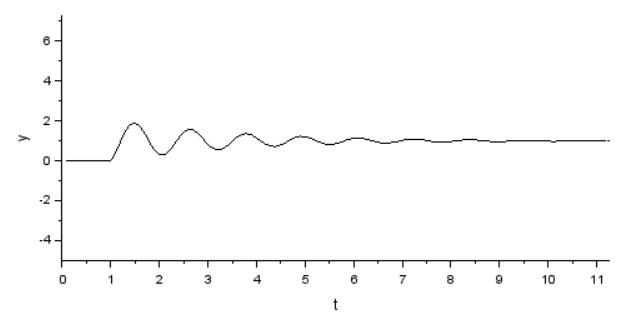
\includegraphics[scale=0.7]{plot1_1}
	\caption{Структурная схема моделирования механической системы масса-пружина }
	\label{p:График1_1}
\end{figure}

\newpage
\section{Исследование модели вход-состояние-выход}

\end{document}